\documentclass[12pt,a4paper]{article}

% ── Packages ──────────────────────────────────────────────────────
\usepackage[margin=2.5cm]{geometry}
\usepackage{graphicx}
\usepackage{hyperref}
\usepackage{listings}
\usepackage{xcolor}
\usepackage{booktabs}
\usepackage{longtable}
\usepackage{enumitem}
\usepackage{fancyhdr}
\usepackage{tikz}
\usetikzlibrary{arrows.meta, positioning, shapes.geometric, fit}
\usepackage{forest}
\usepackage{tabularx}
\usepackage{array}
\usepackage{titlesec}

% ── Colors ────────────────────────────────────────────────────────
\definecolor{codebg}{HTML}{F5F5F5}
\definecolor{codeframe}{HTML}{CCCCCC}
\definecolor{keyword}{HTML}{0077AA}
\definecolor{string}{HTML}{669900}
\definecolor{comment}{HTML}{999999}
\definecolor{routeget}{HTML}{61AFFE}
\definecolor{routepost}{HTML}{49CC90}
\definecolor{routepatch}{HTML}{FCA130}
\definecolor{routedelete}{HTML}{F93E3E}
\definecolor{routeput}{HTML}{9B59B6}

% ── Listing Style ─────────────────────────────────────────────────
\lstdefinestyle{jscode}{
    backgroundcolor=\color{codebg},
    frame=single,
    rulecolor=\color{codeframe},
    basicstyle=\ttfamily\footnotesize,
    keywordstyle=\color{keyword}\bfseries,
    stringstyle=\color{string},
    commentstyle=\color{comment}\itshape,
    breaklines=true,
    tabsize=2,
    showstringspaces=false
}

% ── HTTP method badges ────────────────────────────────────────────
\newcommand{\GET}{\colorbox{routeget}{\texttt{\textbf{\color{white}GET}}}}
\newcommand{\POST}{\colorbox{routepost}{\texttt{\textbf{\color{white}POST}}}}
\newcommand{\PATCH}{\colorbox{routepatch}{\texttt{\textbf{\color{white}PATCH}}}}
\newcommand{\DELETE}{\colorbox{routedelete}{\texttt{\textbf{\color{white}DELETE}}}}
\newcommand{\PUT}{\colorbox{routeput}{\texttt{\textbf{\color{white}PUT}}}}

% ── Header / Footer ──────────────────────────────────────────────
\pagestyle{fancy}
\fancyhf{}
\fancyhead[L]{\small Civic Engagement Platform --- Backend Architecture}
\fancyhead[R]{\small\thepage}
\fancyfoot[C]{\small Civic-Engagement-SE3040-Project}

% ── Title ─────────────────────────────────────────────────────────
\title{%
  \vspace{-1cm}
  \textbf{Civic Engagement Platform}\\[4pt]
  \Large Backend Architecture \& API Documentation
}
\author{SE3040 --- Application Frameworks}
\date{\today}

% ══════════════════════════════════════════════════════════════════
\begin{document}
\maketitle
\tableofcontents
\newpage

% ══════════════════════════════════════════════════════════════════
\section{Project Overview}
% ══════════════════════════════════════════════════════════════════

The \textbf{Civic Engagement Platform} is a Node.js/Express RESTful API that enables citizens, officials, and administrators to interact on civic matters. The backend is built with the following technology stack:

\begin{itemize}[leftmargin=1.5cm]
  \item \textbf{Runtime:} Node.js (ES Modules)
  \item \textbf{Framework:} Express.js v4
  \item \textbf{Database:} MongoDB via Mongoose ODM v8
  \item \textbf{Authentication:} JSON Web Tokens (jsonwebtoken + bcryptjs)
  \item \textbf{File Uploads:} Multer + Cloudinary
  \item \textbf{Email:} Nodemailer
  \item \textbf{Validation:} express-validator
  \item \textbf{Pagination:} mongoose-paginate-v2
  \item \textbf{Testing:} Jest + Supertest
\end{itemize}

The API is versioned under \texttt{/api/v1/} and serves six main modules:
\textbf{Auth}, \textbf{Issues}, \textbf{Marketplace}, \textbf{Surveys}, \textbf{Geocoding}, and \textbf{Green Initiatives}.

% ══════════════════════════════════════════════════════════════════
\section{Directory Structure}
% ══════════════════════════════════════════════════════════════════

\begin{lstlisting}[style=jscode, title={\textbf{Backend File Tree}}]
backend/
|-- server.js                  # Entry point: DB connect + listen
|-- package.json               # Dependencies & scripts
|-- seed.js                    # Database seeding script
|-- src/
|   |-- app.js                 # Express app setup & route mounting
|   |-- config/
|   |   |-- env.js             # Environment variable exports
|   |   |-- database.js        # MongoDB connection
|   |   |-- constants.js       # Roles, statuses, categories
|   |   |-- cloudinary.config.js # Cloudinary + Multer setup
|   |-- middleware/
|   |   |-- auth.middleware.js       # JWT protect & authorize
|   |   |-- error.middleware.js      # Global error handler
|   |   |-- validation.middleware.js # express-validator runner
|   |   |-- logger.middleware.js     # Request logging
|   |-- models/
|   |   |-- User.model.js           # User schema
|   |   |-- Issue.model.js          # Issue schema (GeoJSON)
|   |   |-- Marketplace.model.js    # Marketplace listing schema
|   |   |-- GreenInitiative.model.js # Green initiative schema
|   |   |-- survey.model.js         # Survey schema
|   |   |-- surveyResponse.model.js  # Survey response schema
|   |-- routes/
|   |   |-- auth.routes.js
|   |   |-- issue.routes.js
|   |   |-- marketplace.routes.js
|   |   |-- survey.routes.js
|   |   |-- geocoding.routes.js
|   |   |-- greenInitiative.routes.js
|   |-- controllers/
|   |   |-- auth.controller.js
|   |   |-- issue.controller.js
|   |   |-- marketplace.controller.js
|   |   |-- survey.controller.js
|   |   |-- geocoding.controller.js
|   |   |-- greenInitiative.controller.js
|   |-- services/
|   |   |-- issue.service.js
|   |   |-- marketplace.service.js
|   |   |-- survey.service.js
|   |   |-- geocoding.service.js
|   |   |-- cloudinary.service.js
|   |-- validators/
|   |   |-- issue.validators.js
|   |   |-- marketplace.validators.js
|   |   |-- survey.validator.js
|   |-- utils/
|       |-- AppError.js         # Custom error class
|       |-- asyncHandler.js     # Async/await try-catch wrapper
|       |-- response.js         # Standardized JSON responses
|       |-- mailer.js           # Nodemailer transporter
|-- tests/                     # Jest test suites
\end{lstlisting}

% ══════════════════════════════════════════════════════════════════
\section{Folder-by-Folder Explanation}
% ══════════════════════════════════════════════════════════════════

This section explains the purpose of every folder and what each file inside it does.

% ── 3.1 Root Files ────────────────────────────────────────────────
\subsection{Root Files (\texttt{backend/})}

\begin{itemize}[leftmargin=1cm]
  \item \textbf{\texttt{server.js}} --- The entry point of the entire application. When you run \texttt{npm run dev} or \texttt{npm start}, this file executes first. It does three things: (1) imports the configured Express app from \texttt{src/app.js}, (2) calls \texttt{connectDB()} to connect to MongoDB, and (3) starts the HTTP server on the configured port. It also registers a global \texttt{unhandledRejection} handler that gracefully shuts down the server if an unhandled promise rejection occurs.

  \item \textbf{\texttt{package.json}} --- Defines the project metadata, npm scripts (\texttt{dev}, \texttt{start}, \texttt{test}), all runtime dependencies (express, mongoose, jsonwebtoken, bcryptjs, cloudinary, multer, nodemailer, etc.), and dev dependencies (jest, nodemon, supertest). The project uses ES Modules (\texttt{"type": "module"}).

  \item \textbf{\texttt{seed.js}} --- A standalone script used to populate the MongoDB database with initial sample data (users, issues, listings, etc.) for development and testing purposes.

  \item \textbf{\texttt{src/app.js}} --- Configures the Express application. This is where all global middleware is applied (CORS, JSON body parsing, URL-encoded parsing, Morgan logging) and where all six route modules are mounted under their respective \texttt{/api/v1/} prefixes. It also defines the \texttt{GET /health} endpoint and a 404 catch-all handler. The global error middleware is attached at the very end.
\end{itemize}

% ── 3.2 Config ────────────────────────────────────────────────────
\subsection{\texttt{config/} --- Configuration Layer}

This folder holds all the configuration logic that the rest of the application depends on. No business logic exists here --- only setup and initialization.

\begin{itemize}[leftmargin=1cm]
  \item \textbf{\texttt{env.js}} --- Loads the \texttt{.env} file using the \texttt{dotenv} package and exports all environment variables as named constants (e.g., \texttt{PORT}, \texttt{MONGODB\_URI}, \texttt{JWT\_SECRET}, \texttt{CLOUDINARY\_CLOUD\_NAME}, \texttt{MAIL\_HOST}, etc.). Every other file in the project imports from here instead of reading \texttt{process.env} directly, providing a single source of truth for configuration.

  \item \textbf{\texttt{database.js}} --- Exports a single async function \texttt{connectDB()} that uses Mongoose to connect to MongoDB using the \texttt{MONGODB\_URI} from \texttt{env.js}. If the connection fails, it logs the error and terminates the process with exit code 1.

  \item \textbf{\texttt{constants.js}} --- Defines all application-wide constants as exported objects and arrays:
  \begin{itemize}
    \item \texttt{ROLES}: User role enums (\texttt{citizen}, \texttt{official}, \texttt{admin})
    \item \texttt{STATUS\_CODES}: HTTP status code constants (200, 201, 400, 401, 403, 404, 500)
    \item \texttt{ISSUE\_STATUS}: Issue lifecycle states (\texttt{Pending}, \texttt{In Progress}, \texttt{Resolved}, \texttt{Withdrawn})
    \item \texttt{ISSUE\_CATEGORIES}: Valid issue categories (Pothole, Broken Streetlight, Illegal Dumping, etc.)
    \item \texttt{ALLOWED\_TRANSITIONS}: A state machine map defining which status transitions are valid from each state
    \item \texttt{RESOLVE\_ROLES}: Roles permitted to move an issue to ``Resolved'' status
  \end{itemize}

  \item \textbf{\texttt{cloudinary.config.js}} --- Configures the Cloudinary SDK with credentials from \texttt{env.js}, creates a \texttt{CloudinaryStorage} instance for Multer that stores uploaded images in the \texttt{civic-engagement/issues} folder on Cloudinary (allowing jpg, jpeg, png, webp formats with auto-quality and max 1200$\times$1200 resizing), defines a file filter that only accepts image MIME types, and exports a configured \texttt{multer} upload middleware with a 5\,MB per-file and 5-file-per-request limit.
\end{itemize}

% ── 3.3 Middleware ────────────────────────────────────────────────
\subsection{\texttt{middleware/} --- Request Interceptors}

Middleware functions sit between the incoming request and the route handler. They can modify the request, reject it, or pass it along.

\begin{itemize}[leftmargin=1cm]
  \item \textbf{\texttt{auth.middleware.js}} --- Contains two exported functions:
  \begin{itemize}
    \item \texttt{protect}: Extracts the JWT from the \texttt{Authorization: Bearer <token>} header, verifies it using the HS256 algorithm and the \texttt{JWT\_SECRET}, validates that the decoded payload contains \texttt{id} and \texttt{role} fields, and attaches the decoded user data to \texttt{req.user} (as \texttt{\{id, email, role\}}). If no token is provided or verification fails, it returns a 401 error.
    \item \texttt{authorize(...roles)}: A higher-order function that returns middleware checking whether \texttt{req.user.role} is in the allowed roles list. If not, it returns a 403 Forbidden error.
  \end{itemize}

  \item \textbf{\texttt{error.middleware.js}} --- The global error-handling middleware (4-argument Express middleware). When any error is thrown or passed via \texttt{next(error)} from anywhere in the pipeline, this middleware catches it and sends a standardized JSON response with \texttt{status} and \texttt{message}. In development mode, it also includes the stack trace. In production mode, non-operational errors (unexpected bugs) have their message replaced with a generic ``Internal server error'' to avoid leaking details.

  \item \textbf{\texttt{validation.middleware.js}} --- Runs \texttt{express-validator}'s \texttt{validationResult(req)} to check if any validation rules (defined in the validators folder) have failed. If there are errors, it immediately returns a 400 response with an array of all validation error messages. If no errors, it calls \texttt{next()} to proceed.

  \item \textbf{\texttt{logger.middleware.js}} --- A simple custom request logger that prints a timestamp, HTTP method, and request path to the console for every incoming request. This supplements the Morgan logger used in \texttt{app.js}.
\end{itemize}

% ── 3.4 Models ────────────────────────────────────────────────────
\subsection{\texttt{models/} --- Mongoose Schemas \& Data Layer}

Each file in this folder defines a Mongoose schema that maps to a MongoDB collection. The schemas include field types, validations, defaults, indexes, and plugins.

\begin{itemize}[leftmargin=1cm]
  \item \textbf{\texttt{User.model.js}} --- Defines the \texttt{User} schema with fields: \texttt{name} (String, max 50), \texttt{email} (String, unique, lowercase), \texttt{password} (String, min 6 chars --- stored as a bcrypt hash), and \texttt{role} (enum: \texttt{user}/\texttt{admin}/\texttt{official}, default \texttt{user}). Includes auto-generated \texttt{createdAt}/\texttt{updatedAt} timestamps.

  \item \textbf{\texttt{Issue.model.js}} --- The most complex model. Defines the \texttt{Issue} schema with sub-schemas for \texttt{statusHistory} (audit trail of status changes with who changed it and when), \texttt{comments} (admin/official comments), and \texttt{images} (Cloudinary URL + public ID pairs, max 5). The \texttt{location} field uses GeoJSON \texttt{Point} format with coordinate validation. Includes four database indexes: a 2dsphere geospatial index for map queries, and compound indexes for optimizing common queries by reporter, status/category, and date. Uses the \texttt{mongoose-paginate-v2} plugin for paginated queries.

  \item \textbf{\texttt{Marketplace.model.js}} --- Defines a marketplace listing with \texttt{title}, \texttt{description}, \texttt{category} (free text), \texttt{type} (donation or sale), \texttt{price} (required only for sales), \texttt{images} (array of URL strings), \texttt{status} (available/reserved/sold/expired), \texttt{owner} (ObjectId reference to User), \texttt{contactInfo}, and \texttt{expiresAt} (auto-set to 30 days from creation).

  \item \textbf{\texttt{GreenInitiative.model.js}} --- Defines a community green initiative with \texttt{title}, \texttt{description}, \texttt{location} (plain string), \texttt{date}, \texttt{status} (Upcoming/Ongoing/Completed), \texttt{organizer} (stored as a String user ID), and \texttt{participants} (array of String user IDs).

  \item \textbf{\texttt{survey.model.js}} --- Defines surveys with a sub-schema for \texttt{options} (each option has a \texttt{text} and \texttt{voteCount}), plus \texttt{title}, \texttt{description}, \texttt{deadline}, \texttt{targetAudience} (all/citizen/official), \texttt{status} (active/closed/expired), \texttt{isImportant} flag, \texttt{createdBy}, and \texttt{totalVotes}. Has a Mongoose \texttt{pre('find')} middleware hook that automatically filters out expired surveys from query results.

  \item \textbf{\texttt{surveyResponse.model.js}} --- Tracks individual votes. Each response records a \texttt{surveyId} (ObjectId reference), \texttt{userId} (String), and \texttt{selectedOptionIndex} (Number). A unique compound index on \texttt{(surveyId, userId)} enforces one vote per user per survey at the database level.
\end{itemize}

% ── 3.5 Routes ────────────────────────────────────────────────────
\subsection{\texttt{routes/} --- URL-to-Handler Mapping}

Each file in this folder creates an Express \texttt{Router}, defines the HTTP endpoints (GET, POST, PATCH, PUT, DELETE), attaches the appropriate middleware chain (authentication, authorization, validation), and maps each endpoint to the correct controller function.

\begin{itemize}[leftmargin=1cm]
  \item \textbf{\texttt{auth.routes.js}} --- Mounts 3 endpoints under \texttt{/api/v1/auth}: \texttt{POST /register} and \texttt{POST /login} (both public), and \texttt{GET /me} (protected with the \texttt{protect} middleware).

  \item \textbf{\texttt{issue.routes.js}} --- Mounts 8 endpoints under \texttt{/api/v1/issues}. Routes are organized by access level following the Interface Segregation Principle: public routes first (\texttt{GET /} and \texttt{GET /:id}), then authenticated routes (\texttt{GET /my-issues}, \texttt{POST /}, \texttt{PATCH /:id/withdraw}, \texttt{DELETE /:id}), then admin/official-only routes (\texttt{PATCH /:id/status}, \texttt{POST /:id/comments}). Uses the Cloudinary upload middleware on the create endpoint to accept up to 5 images. Each route applies the relevant validators before the controller.

  \item \textbf{\texttt{marketplace.routes.js}} --- Mounts 6 endpoints under \texttt{/api/v1/marketplace}. Public routes for browsing (\texttt{GET /} and \texttt{GET /:id}), and authenticated routes for managing listings (\texttt{POST /}, \texttt{PATCH /:id}, \texttt{PATCH /:id/status}, \texttt{DELETE /:id}). Each route applies marketplace-specific validators.

  \item \textbf{\texttt{greenInitiative.routes.js}} --- Mounts 5 endpoints under \texttt{/api/v1/green-initiatives} using Express route chaining (\texttt{router.route('/')}). Public GET routes and protected POST/PUT/DELETE routes. Does not use separate validators.

  \item \textbf{\texttt{survey.routes.js}} --- Mounts 7 endpoints under \texttt{/api/v1/surveys}. All routes require authentication. Creation, update, and deletion are restricted to admin/official roles using the \texttt{authorize} middleware with role constants from \texttt{constants.js}. Voting is open to all authenticated roles.

  \item \textbf{\texttt{geocoding.routes.js}} --- Mounts 2 public endpoints under \texttt{/api/v1/geocode}: \texttt{GET /reverse} (coordinates $\rightarrow$ address) and \texttt{GET /forward} (address $\rightarrow$ coordinates). Inline \texttt{express-validator} query parameter validation is defined directly in the route file (lat must be $-90$ to $90$, lng must be $-180$ to $180$, address must be 2--300 characters).
\end{itemize}

% ── 3.6 Controllers ──────────────────────────────────────────────
\subsection{\texttt{controllers/} --- HTTP Request/Response Handlers}

Controllers are thin layer functions that extract data from the request (\texttt{req.body}, \texttt{req.params}, \texttt{req.query}, \texttt{req.user}), call the appropriate service or model method, and send a standardized JSON response using the \texttt{sendSuccess} utility. They contain no business logic.

\begin{itemize}[leftmargin=1cm]
  \item \textbf{\texttt{auth.controller.js}} --- Handles user registration (hash password with bcryptjs, create user in DB, sign JWT), login (find user by email, compare password hashes, sign JWT), and \texttt{getMe} (return current user from token). This is the only controller that directly interacts with the model (no separate service layer) because auth logic is self-contained.

  \item \textbf{\texttt{issue.controller.js}} --- Delegates all logic to \texttt{IssueService}. Handles: \texttt{createIssue} (passes body, user ID, and uploaded files), \texttt{getMyIssues}, \texttt{getPublicIssues}, \texttt{getIssueById}, \texttt{updateStatus} (extracts status and comment from body), \texttt{addComment}, \texttt{withdrawIssue}, and \texttt{deleteIssue}.

  \item \textbf{\texttt{marketplace.controller.js}} --- Delegates all logic to \texttt{MarketplaceService}. Handles: \texttt{createListing}, \texttt{getAllListings}, \texttt{getListingById}, \texttt{updateListing}, \texttt{updateListingStatus}, and \texttt{deleteListing}. Passes the full \texttt{req.user} object to the service for ownership checks.

  \item \textbf{\texttt{survey.controller.js}} --- Delegates all logic to \texttt{SurveyService}. Handles: \texttt{createSurvey}, \texttt{getActiveSurveys} (passes user role for audience filtering), \texttt{getSurveyById}, \texttt{voteOnSurvey} (passes selected option index), \texttt{updateSurvey}, \texttt{deleteSurvey}, and \texttt{getSurveyResults}.

  \item \textbf{\texttt{geocoding.controller.js}} --- Delegates to \texttt{GeocodingService}. Handles: \texttt{reverseGeocode} (parses lat/lng from query params) and \texttt{forwardGeocode} (passes address string).

  \item \textbf{\texttt{greenInitiative.controller.js}} --- Directly interacts with the \texttt{GreenInitiative} Mongoose model (no service layer). Handles CRUD operations with inline authorization checks (verifying the requester is the organizer or an admin before allowing updates/deletes).
\end{itemize}

% ── 3.7 Services ─────────────────────────────────────────────────
\subsection{\texttt{services/} --- Business Logic Layer}

Services contain all the business rules, data transformations, and complex operations. They interact with models and external APIs. Controllers call services; services never touch \texttt{req} or \texttt{res} directly.

\begin{itemize}[leftmargin=1cm]
  \item \textbf{\texttt{issue.service.js}} --- The largest service file. Contains business logic for: creating issues (mapping uploaded files to Cloudinary URLs, building the GeoJSON location object, initializing status history), retrieving user issues and public issues (with filtering by status/category and pagination), getting a single issue by ID, updating issue status (validates allowed transitions using the \texttt{ALLOWED\_TRANSITIONS} map from constants, checks role permissions for resolving, appends to the status history audit trail), adding comments, withdrawing issues (only the original reporter can withdraw), and deleting issues (reporter or admin only).

  \item \textbf{\texttt{marketplace.service.js}} --- Handles: creating listings (attaching owner from user ID), retrieving all listings (with filtering by category/type/status and pagination), getting a single listing, updating listing fields (with ownership verification --- only the owner or an admin can edit), updating listing status, and deleting listings.

  \item \textbf{\texttt{survey.service.js}} --- Handles: creating surveys (saving to DB), fetching active surveys (filtering by target audience based on user role), getting a single survey, voting (checks if user already voted via \texttt{SurveyResponse}, increments the option's \texttt{voteCount} and the survey's \texttt{totalVotes}), updating survey details, closing/deleting surveys, and fetching aggregated survey results formatted for Chart.js visualization.

  \item \textbf{\texttt{geocoding.service.js}} --- Interacts with an external geocoding API (e.g., OpenStreetMap Nominatim or a similar provider). Contains two methods: \texttt{reverseGeocode(lat, lng)} that converts geographic coordinates into a human-readable address, and \texttt{forwardGeocode(address)} that converts an address string into latitude/longitude coordinates.

  \item \textbf{\texttt{cloudinary.service.js}} --- Provides helper functions for interacting with the Cloudinary API beyond what the Multer integration handles. Used by the issue service for managing uploaded images (e.g., deleting images from Cloudinary when an issue is deleted).
\end{itemize}

% ── 3.8 Validators ───────────────────────────────────────────────
\subsection{\texttt{validators/} --- Input Validation Rules}

Each file exports arrays of \texttt{express-validator} validation chains that are applied as middleware in the route files. They run before the controller and check that the request body, params, or query parameters meet expected formats.

\begin{itemize}[leftmargin=1cm]
  \item \textbf{\texttt{issue.validators.js}} --- Defines validation rules for: creating an issue (\texttt{title} is required and max 100 chars, \texttt{description} is required and max 1000 chars, \texttt{category} must be one of the \texttt{ISSUE\_CATEGORIES}, coordinates must be valid numbers within geographic bounds), updating issue status (\texttt{status} must be a valid \texttt{ISSUE\_STATUS} value), adding a comment (\texttt{text} is required, max 500 chars), fetching public issues (optional query filters), and validating the \texttt{:id} param is a valid MongoDB ObjectId.

  \item \textbf{\texttt{marketplace.validators.js}} --- Defines validation rules for: creating a listing (\texttt{title}, \texttt{description}, \texttt{category}, \texttt{type}, \texttt{contactInfo} are required; \texttt{price} is required and non-negative when type is \texttt{sale}), updating a listing (all fields optional but validated if present), updating listing status (\texttt{status} must be one of available/reserved/sold/expired), and validating the \texttt{:id} param.

  \item \textbf{\texttt{survey.validator.js}} --- Defines validation rules for: creating a survey (\texttt{title} required max 150, \texttt{description} required, \texttt{options} must be an array with at least 2 items, \texttt{deadline} must be a valid future date) and voting (\texttt{selectedOptionIndex} must be a non-negative integer).
\end{itemize}

% ── 3.9 Utils ────────────────────────────────────────────────────
\subsection{\texttt{utils/} --- Shared Utility Functions}

This folder contains reusable helper modules that are used across multiple layers of the application.

\begin{itemize}[leftmargin=1cm]
  \item \textbf{\texttt{AppError.js}} --- Defines a custom \texttt{AppError} class that extends the native JavaScript \texttt{Error}. It adds a \texttt{statusCode} (e.g., 400, 404), a \texttt{status} string (\texttt{'fail'} for 4xx codes, \texttt{'error'} for 5xx codes), and an \texttt{isOperational} flag set to \texttt{true}. The error middleware uses \texttt{isOperational} to distinguish between expected application errors (show to user) and unexpected bugs (hide details in production).

  \item \textbf{\texttt{asyncHandler.js}} --- A higher-order function that wraps async Express route handlers. Instead of writing \texttt{try/catch} blocks in every controller, you wrap the function with \texttt{asyncHandler(fn)}. It catches any rejected promises and automatically passes the error to Express's \texttt{next()} function, which triggers the error middleware.

  \item \textbf{\texttt{response.js}} --- Exports two functions for standardized JSON responses:
  \begin{itemize}
    \item \texttt{sendSuccess(res, statusCode, data, message)}: Returns \texttt{\{status: 'success', message, data\}}
    \item \texttt{sendError(res, statusCode, message)}: Returns \texttt{\{status: 'error', message\}}
  \end{itemize}
  This ensures every API response follows the same shape, making the API predictable for frontend consumers.

  \item \textbf{\texttt{mailer.js}} --- Creates a Nodemailer SMTP transporter using credentials from \texttt{env.js} and exports two email-sending functions:
  \begin{itemize}
    \item \texttt{sendNewSurveyNotification(toEmail, surveyTitle, surveyId)}: Sends an HTML email notifying citizens about a new important survey with a ``Vote Now'' button linking to the frontend.
    \item \texttt{sendSurveyClosingReminder(toEmail, surveyTitle, deadline)}: Sends an HTML email reminding users that a survey is about to close, showing the deadline date.
  \end{itemize}
\end{itemize}

% ── 3.10 Tests ───────────────────────────────────────────────────
\subsection{\texttt{tests/} --- Test Suites}

Contains Jest test files that test the API endpoints using Supertest (HTTP integration tests). Tests cover authentication flows, CRUD operations for each module, validation error handling, and role-based access control enforcement.

% ══════════════════════════════════════════════════════════════════
\section{Application Bootstrap Flow}
% ══════════════════════════════════════════════════════════════════

The application starts from \texttt{server.js}, which:

\begin{enumerate}
  \item Imports the Express app from \texttt{src/app.js}
  \item Calls \texttt{connectDB()} to establish a MongoDB connection
  \item Starts the HTTP server on the configured \texttt{PORT}
  \item Registers an \texttt{unhandledRejection} handler for graceful shutdown
\end{enumerate}

\texttt{src/app.js} configures the Express application:

\begin{enumerate}
  \item Applies CORS with configurable origin
  \item Parses JSON and URL-encoded bodies
  \item Enables Morgan HTTP request logging
  \item Mounts all six API route modules
  \item Registers a health-check endpoint (\texttt{GET /health})
  \item Adds a 404 catch-all handler
  \item Applies the global error middleware
\end{enumerate}

% ══════════════════════════════════════════════════════════════════
\section{Request Processing Pipeline}
% ══════════════════════════════════════════════════════════════════

Every incoming request passes through a layered middleware pipeline before reaching the business logic:

\begin{center}
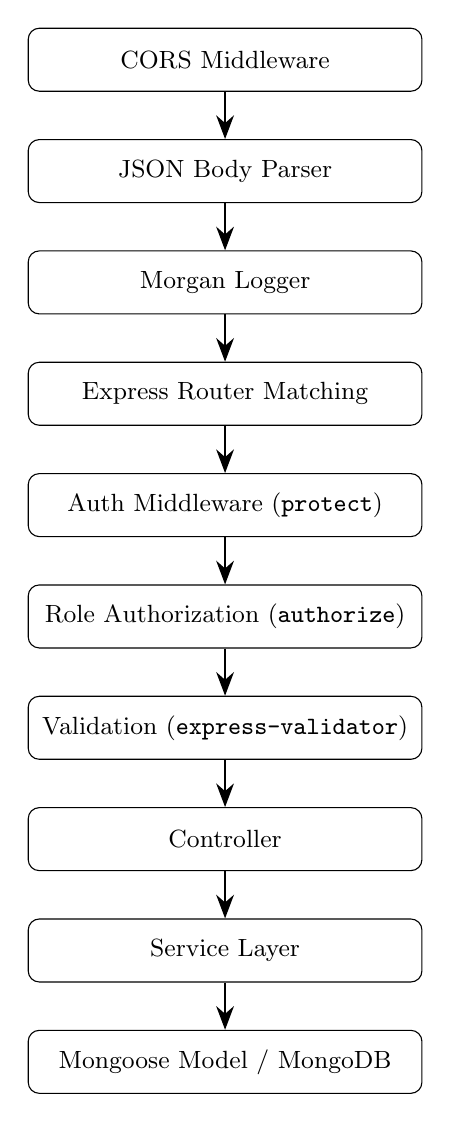
\begin{tikzpicture}[
    node distance=0.6cm,
    every node/.style={draw, rounded corners, minimum width=5cm, minimum height=0.8cm, align=center, font=\small},
    arrow/.style={-{Stealth[length=3mm]}, thick}
]
    \node (cors) {CORS Middleware};
    \node (json) [below=of cors] {JSON Body Parser};
    \node (morgan) [below=of json] {Morgan Logger};
    \node (router) [below=of morgan] {Express Router Matching};
    \node (auth) [below=of router] {Auth Middleware (\texttt{protect})};
    \node (rbac) [below=of auth] {Role Authorization (\texttt{authorize})};
    \node (valid) [below=of rbac] {Validation (\texttt{express-validator})};
    \node (ctrl) [below=of valid] {Controller};
    \node (svc) [below=of ctrl] {Service Layer};
    \node (model) [below=of svc] {Mongoose Model / MongoDB};

    \draw[arrow] (cors) -- (json);
    \draw[arrow] (json) -- (morgan);
    \draw[arrow] (morgan) -- (router);
    \draw[arrow] (router) -- (auth);
    \draw[arrow] (auth) -- (rbac);
    \draw[arrow] (rbac) -- (valid);
    \draw[arrow] (valid) -- (ctrl);
    \draw[arrow] (ctrl) -- (svc);
    \draw[arrow] (svc) -- (model);
\end{tikzpicture}
\end{center}

\noindent\textbf{Note:} Public routes skip the Auth and Authorization middleware steps. The error middleware catches any uncaught errors at any layer and returns a standardized JSON response.

% ══════════════════════════════════════════════════════════════════
\section{Data Models}
% ══════════════════════════════════════════════════════════════════

% ── 5.1 User ──────────────────────────────────────────────────────
\subsection{User Model}

\begin{longtable}{@{}llp{6cm}@{}}
\toprule
\textbf{Field} & \textbf{Type} & \textbf{Description} \\
\midrule
\endhead
\texttt{name}     & String  & Required, max 50 chars, trimmed \\
\texttt{email}    & String  & Required, unique, lowercase \\
\texttt{password} & String  & Required, min 6 chars (bcrypt hashed) \\
\texttt{role}     & String  & Enum: \texttt{user}, \texttt{admin}, \texttt{official} (default: \texttt{user}) \\
\texttt{createdAt / updatedAt} & Date & Auto-generated timestamps \\
\bottomrule
\end{longtable}

% ── 5.2 Issue ─────────────────────────────────────────────────────
\subsection{Issue Model}

\begin{longtable}{@{}llp{5.5cm}@{}}
\toprule
\textbf{Field} & \textbf{Type} & \textbf{Description} \\
\midrule
\endhead
\texttt{title}       & String  & Required, max 100 chars \\
\texttt{description} & String  & Required, max 1000 chars \\
\texttt{category}    & String  & Enum: Pothole, Broken Streetlight, Illegal Dumping, Water Leak, Damaged Sidewalk, Graffiti, Traffic Signal, Other \\
\texttt{status}      & String  & Enum: Pending, In Progress, Resolved, Withdrawn (default: Pending) \\
\texttt{location}    & GeoJSON & \texttt{Point} type with coordinates \texttt{[lng, lat]}, plus optional address string \\
\texttt{images}      & [Object] & Array of \texttt{\{url, publicId\}} (max 5, Cloudinary) \\
\texttt{reporter}    & String  & User ID of the reporter \\
\texttt{statusHistory} & [Object] & Audit trail: \texttt{\{status, changedBy, comment, timestamp\}} \\
\texttt{comments}    & [Object] & \texttt{\{user, text, timestamp\}} \\
\bottomrule
\end{longtable}

\noindent\textbf{Indexes:} 2dsphere on \texttt{location}, compound on \texttt{(reporter, createdAt)}, \texttt{(status, category)}, and \texttt{createdAt}. Pagination via \texttt{mongoose-paginate-v2}.

% ── 5.3 Marketplace ──────────────────────────────────────────────
\subsection{Marketplace Model}

\begin{longtable}{@{}llp{5.5cm}@{}}
\toprule
\textbf{Field} & \textbf{Type} & \textbf{Description} \\
\midrule
\endhead
\texttt{title}       & String   & Required, max 100 chars \\
\texttt{description} & String   & Required, max 1000 chars \\
\texttt{category}    & String   & Free-text category \\
\texttt{type}        & String   & Enum: \texttt{donation}, \texttt{sale} \\
\texttt{price}       & Number   & Required only when type = \texttt{sale}, min 0 \\
\texttt{images}      & [String] & Array of image URLs \\
\texttt{status}      & String   & Enum: \texttt{available}, \texttt{reserved}, \texttt{sold}, \texttt{expired} \\
\texttt{owner}       & ObjectId & Reference to User model \\
\texttt{contactInfo} & String   & Required contact information \\
\texttt{expiresAt}   & Date     & Default: 30 days from creation \\
\bottomrule
\end{longtable}

% ── 5.4 Green Initiative ─────────────────────────────────────────
\subsection{Green Initiative Model}

\begin{longtable}{@{}llp{5.5cm}@{}}
\toprule
\textbf{Field} & \textbf{Type} & \textbf{Description} \\
\midrule
\endhead
\texttt{title}        & String   & Required, max 100 chars \\
\texttt{description}  & String   & Required, max 1000 chars \\
\texttt{location}     & String   & Location name (free text) \\
\texttt{date}         & Date     & Event date \\
\texttt{status}       & String   & Enum: Upcoming, Ongoing, Completed \\
\texttt{organizer}    & String   & User ID of the organizer \\
\texttt{participants} & [String] & Array of participant user IDs \\
\bottomrule
\end{longtable}

% ── 5.5 Survey ────────────────────────────────────────────────────
\subsection{Survey Model}

\begin{longtable}{@{}llp{5.5cm}@{}}
\toprule
\textbf{Field} & \textbf{Type} & \textbf{Description} \\
\midrule
\endhead
\texttt{title}          & String   & Required, max 150 chars \\
\texttt{description}    & String   & Required \\
\texttt{options}        & [Object] & Each has \texttt{text} (String) and \texttt{voteCount} (Number), minimum 2 options \\
\texttt{deadline}       & Date     & Required survey deadline \\
\texttt{targetAudience} & String   & Enum: \texttt{all}, \texttt{citizen}, \texttt{official} \\
\texttt{status}         & String   & Enum: \texttt{active}, \texttt{closed}, \texttt{expired} \\
\texttt{isImportant}    & Boolean  & Flag for priority surveys \\
\texttt{createdBy}      & String   & Creator's user ID \\
\texttt{totalVotes}     & Number   & Running vote count \\
\bottomrule
\end{longtable}

\noindent\textbf{Note:} A \texttt{pre('find')} hook auto-filters expired surveys.

% ── 5.6 Survey Response ──────────────────────────────────────────
\subsection{Survey Response Model}

\begin{longtable}{@{}llp{5.5cm}@{}}
\toprule
\textbf{Field} & \textbf{Type} & \textbf{Description} \\
\midrule
\endhead
\texttt{surveyId}            & ObjectId & Reference to Survey \\
\texttt{userId}              & String   & Voter's user ID \\
\texttt{selectedOptionIndex} & Number   & Index of the chosen option \\
\bottomrule
\end{longtable}

\noindent\textbf{Constraint:} Unique compound index on \texttt{(surveyId, userId)} ensures one vote per user per survey.

% ══════════════════════════════════════════════════════════════════
\section{Middleware Layer}
% ══════════════════════════════════════════════════════════════════

\subsection{Authentication (\texttt{auth.middleware.js})}

\begin{itemize}
  \item \texttt{protect}: Extracts Bearer token from \texttt{Authorization} header, verifies with HS256 algorithm, and attaches \texttt{req.user = \{id, email, role\}} to the request.
  \item \texttt{authorize(...roles)}: Checks if \texttt{req.user.role} is in the allowed roles list; returns 403 if not.
\end{itemize}

\subsection{Validation (\texttt{validation.middleware.js})}
Runs \texttt{express-validator}'s \texttt{validationResult()} and returns a 400 response with all validation errors if any exist.

\subsection{Error Handling (\texttt{error.middleware.js})}
Global error middleware that catches all errors (including those from \texttt{AppError}) and returns a standardized JSON error response.

% ══════════════════════════════════════════════════════════════════
\section{API Endpoints}
% ══════════════════════════════════════════════════════════════════

% ── 7.1 Auth ──────────────────────────────────────────────────────
\subsection{Authentication --- \texttt{/api/v1/auth}}

\begin{longtable}{@{}p{1cm}p{4cm}p{2.5cm}p{5.5cm}@{}}
\toprule
\textbf{Method} & \textbf{Endpoint} & \textbf{Access} & \textbf{Description} \\
\midrule
\endhead
\POST  & \texttt{/register} & Public & Register a new user. Body: \texttt{\{name, email, password, role?\}}. Returns user object + JWT token. \\[6pt]
\POST  & \texttt{/login}    & Public & Login with credentials. Body: \texttt{\{email, password\}}. Returns user object + JWT token. \\[6pt]
\GET   & \texttt{/me}       & Protected & Get the currently authenticated user's profile. Requires Bearer token. \\
\bottomrule
\end{longtable}

\noindent\textbf{Integration Flow:}
\begin{center}
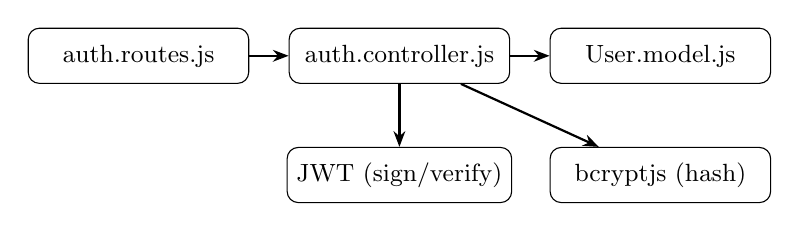
\begin{tikzpicture}[
    node distance=0.8cm and 0.5cm,
    box/.style={draw, rounded corners, minimum width=2.8cm, minimum height=0.7cm, align=center, font=\small},
    arrow/.style={-{Stealth[length=2mm]}, thick}
]
    \node[box] (route) {auth.routes.js};
    \node[box, right=of route] (ctrl) {auth.controller.js};
    \node[box, right=of ctrl] (model) {User.model.js};
    \node[box, below=of ctrl] (jwt) {JWT (sign/verify)};
    \node[box, below=of model] (bcrypt) {bcryptjs (hash)};

    \draw[arrow] (route) -- (ctrl);
    \draw[arrow] (ctrl) -- (model);
    \draw[arrow] (ctrl) -- (jwt);
    \draw[arrow] (ctrl) -- (bcrypt);
\end{tikzpicture}
\end{center}

% ── 7.2 Issues ────────────────────────────────────────────────────
\subsection{Issue Reporting --- \texttt{/api/v1/issues}}

\begin{longtable}{@{}p{1.2cm}p{4cm}p{2.8cm}p{4.5cm}@{}}
\toprule
\textbf{Method} & \textbf{Endpoint} & \textbf{Access} & \textbf{Description} \\
\midrule
\endhead
\GET    & \texttt{/}              & Public             & Get all public issues (filtered, paginated) \\[4pt]
\GET    & \texttt{/my-issues}     & Protected          & Get the authenticated user's issues \\[4pt]
\GET    & \texttt{/:id}           & Public             & Get a single issue by ID \\[4pt]
\POST   & \texttt{/}              & Protected          & Create a new issue (supports up to 5 image uploads via Cloudinary) \\[4pt]
\PATCH  & \texttt{/:id/withdraw}  & Protected (reporter) & Withdraw an issue (reporter only) \\[4pt]
\DELETE & \texttt{/:id}           & Protected          & Delete an issue (reporter or admin) \\[4pt]
\PATCH  & \texttt{/:id/status}    & Admin/Official     & Update issue status with optional comment \\[4pt]
\POST   & \texttt{/:id/comments}  & Admin/Official     & Add a comment to an issue \\
\bottomrule
\end{longtable}

\noindent\textbf{Status Transitions:}
\begin{center}
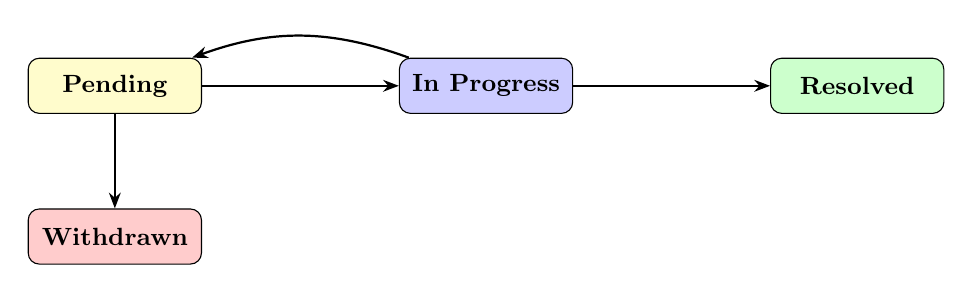
\begin{tikzpicture}[
    state/.style={draw, rounded corners, minimum width=2.2cm, minimum height=0.7cm, align=center, font=\small\bfseries},
    arrow/.style={-{Stealth[length=2mm]}, thick}
]
    \node[state, fill=yellow!20]  (pending) {Pending};
    \node[state, fill=blue!20, right=2.5cm of pending]   (inprog) {In Progress};
    \node[state, fill=green!20, right=2.5cm of inprog]   (resolved) {Resolved};
    \node[state, fill=red!20, below=1.2cm of pending]     (withdrawn) {Withdrawn};

    \draw[arrow] (pending) -- (inprog);
    \draw[arrow] (inprog) -- (resolved);
    \draw[arrow] (inprog) to[bend right=20] (pending);
    \draw[arrow] (pending) -- (withdrawn);
\end{tikzpicture}
\end{center}

\noindent\textbf{Integration Flow:}
\begin{center}
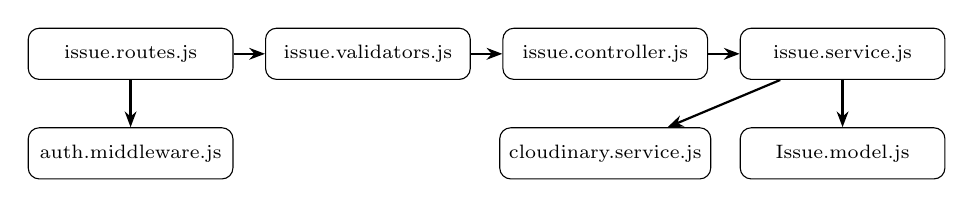
\begin{tikzpicture}[
    node distance=0.5cm and 0.4cm,
    box/.style={draw, rounded corners, minimum width=2.6cm, minimum height=0.65cm, align=center, font=\scriptsize},
    arrow/.style={-{Stealth[length=2mm]}, thick}
]
    \node[box] (route) {issue.routes.js};
    \node[box, right=of route] (valid) {issue.validators.js};
    \node[box, right=of valid] (ctrl) {issue.controller.js};
    \node[box, right=of ctrl] (svc) {issue.service.js};
    \node[box, below=0.6cm of svc] (model) {Issue.model.js};
    \node[box, below=0.6cm of ctrl] (cloud) {cloudinary.service.js};
    \node[box, below=0.6cm of route] (auth) {auth.middleware.js};

    \draw[arrow] (route) -- (valid);
    \draw[arrow] (valid) -- (ctrl);
    \draw[arrow] (ctrl) -- (svc);
    \draw[arrow] (svc) -- (model);
    \draw[arrow] (svc) -- (cloud);
    \draw[arrow] (route) -- (auth);
\end{tikzpicture}
\end{center}

% ── 7.3 Marketplace ──────────────────────────────────────────────
\subsection{Marketplace --- \texttt{/api/v1/marketplace}}

\begin{longtable}{@{}p{1.2cm}p{4cm}p{2.8cm}p{4.5cm}@{}}
\toprule
\textbf{Method} & \textbf{Endpoint} & \textbf{Access} & \textbf{Description} \\
\midrule
\endhead
\GET    & \texttt{/}            & Public    & Get all listings (filtered, paginated) \\[4pt]
\GET    & \texttt{/:id}         & Public    & Get a single listing by ID \\[4pt]
\POST   & \texttt{/}            & Protected & Create a new listing \\[4pt]
\PATCH  & \texttt{/:id}         & Protected & Update a listing (owner/admin) \\[4pt]
\PATCH  & \texttt{/:id/status}  & Protected & Update listing status (owner/admin) \\[4pt]
\DELETE & \texttt{/:id}         & Protected & Delete a listing (owner/admin) \\
\bottomrule
\end{longtable}

\noindent\textbf{Integration Flow:}
\begin{center}
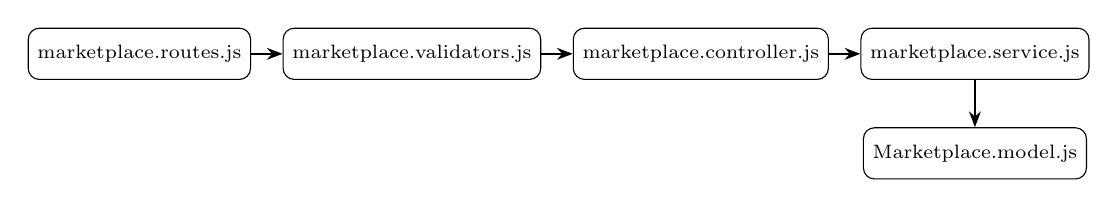
\begin{tikzpicture}[
    node distance=0.5cm and 0.4cm,
    box/.style={draw, rounded corners, minimum width=2.8cm, minimum height=0.65cm, align=center, font=\scriptsize},
    arrow/.style={-{Stealth[length=2mm]}, thick}
]
    \node[box] (route) {marketplace.routes.js};
    \node[box, right=of route] (valid) {marketplace.validators.js};
    \node[box, right=of valid] (ctrl) {marketplace.controller.js};
    \node[box, right=of ctrl] (svc) {marketplace.service.js};
    \node[box, below=0.6cm of svc] (model) {Marketplace.model.js};

    \draw[arrow] (route) -- (valid);
    \draw[arrow] (valid) -- (ctrl);
    \draw[arrow] (ctrl) -- (svc);
    \draw[arrow] (svc) -- (model);
\end{tikzpicture}
\end{center}

% ── 7.4 Green Initiatives ────────────────────────────────────────
\subsection{Green Initiatives --- \texttt{/api/v1/green-initiatives}}

\begin{longtable}{@{}p{1.2cm}p{4cm}p{2.8cm}p{4.5cm}@{}}
\toprule
\textbf{Method} & \textbf{Endpoint} & \textbf{Access} & \textbf{Description} \\
\midrule
\endhead
\POST   & \texttt{/}    & Protected & Create a new green initiative \\[4pt]
\GET    & \texttt{/}    & Public    & Get all green initiatives \\[4pt]
\GET    & \texttt{/:id} & Public    & Get a single initiative by ID \\[4pt]
\PUT    & \texttt{/:id} & Protected & Update an initiative (organizer/admin) \\[4pt]
\DELETE & \texttt{/:id} & Protected & Delete an initiative (organizer/admin) \\
\bottomrule
\end{longtable}

\noindent\textbf{Integration Flow:}
\begin{center}
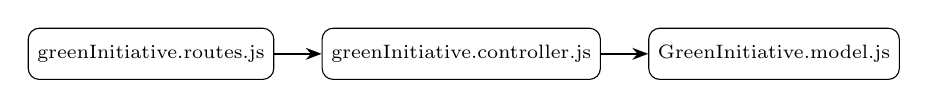
\begin{tikzpicture}[
    node distance=0.5cm and 0.6cm,
    box/.style={draw, rounded corners, minimum width=3cm, minimum height=0.65cm, align=center, font=\scriptsize},
    arrow/.style={-{Stealth[length=2mm]}, thick}
]
    \node[box] (route) {greenInitiative.routes.js};
    \node[box, right=of route] (ctrl) {greenInitiative.controller.js};
    \node[box, right=of ctrl] (model) {GreenInitiative.model.js};

    \draw[arrow] (route) -- (ctrl);
    \draw[arrow] (ctrl) -- (model);
\end{tikzpicture}
\end{center}

\noindent\textbf{Note:} The Green Initiative controller interacts directly with the Mongoose model (no separate service layer). Authorization is checked inline in the controller.

% ── 7.5 Surveys ──────────────────────────────────────────────────
\subsection{Surveys --- \texttt{/api/v1/surveys}}

\begin{longtable}{@{}p{1.2cm}p{4cm}p{2.8cm}p{4.5cm}@{}}
\toprule
\textbf{Method} & \textbf{Endpoint} & \textbf{Access} & \textbf{Description} \\
\midrule
\endhead
\POST   & \texttt{/}             & Admin/Official        & Create a new survey \\[4pt]
\GET    & \texttt{/active}       & All Authenticated     & Get all active surveys \\[4pt]
\GET    & \texttt{/:id}          & All Authenticated     & Get a single survey \\[4pt]
\GET    & \texttt{/:id/results}  & All Authenticated     & Get survey results (for Chart.js) \\[4pt]
\PATCH  & \texttt{/:id/vote}     & All Authenticated     & Cast a vote on a survey \\[4pt]
\PUT    & \texttt{/:id}          & Admin/Official        & Update a survey \\[4pt]
\DELETE & \texttt{/:id}          & Admin/Official        & Close/delete a survey \\
\bottomrule
\end{longtable}

\noindent\textbf{Integration Flow:}
\begin{center}
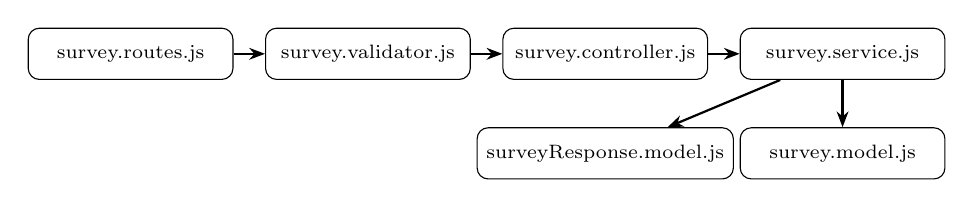
\begin{tikzpicture}[
    node distance=0.5cm and 0.4cm,
    box/.style={draw, rounded corners, minimum width=2.6cm, minimum height=0.65cm, align=center, font=\scriptsize},
    arrow/.style={-{Stealth[length=2mm]}, thick}
]
    \node[box] (route) {survey.routes.js};
    \node[box, right=of route] (valid) {survey.validator.js};
    \node[box, right=of valid] (ctrl) {survey.controller.js};
    \node[box, right=of ctrl] (svc) {survey.service.js};
    \node[box, below=0.6cm of svc] (model) {survey.model.js};
    \node[box, below=0.6cm of ctrl] (resp) {surveyResponse.model.js};

    \draw[arrow] (route) -- (valid);
    \draw[arrow] (valid) -- (ctrl);
    \draw[arrow] (ctrl) -- (svc);
    \draw[arrow] (svc) -- (model);
    \draw[arrow] (svc) -- (resp);
\end{tikzpicture}
\end{center}

% ── 7.6 Geocoding ────────────────────────────────────────────────
\subsection{Geocoding --- \texttt{/api/v1/geocode}}

\begin{longtable}{@{}p{1cm}p{5cm}p{2cm}p{4.5cm}@{}}
\toprule
\textbf{Method} & \textbf{Endpoint} & \textbf{Access} & \textbf{Description} \\
\midrule
\endhead
\GET & \texttt{/reverse?lat=\&lng=} & Public & Convert coordinates to address (reverse geocode) \\[4pt]
\GET & \texttt{/forward?address=}   & Public & Convert address to coordinates (forward geocode) \\
\bottomrule
\end{longtable}

\noindent\textbf{Integration Flow:}
\begin{center}
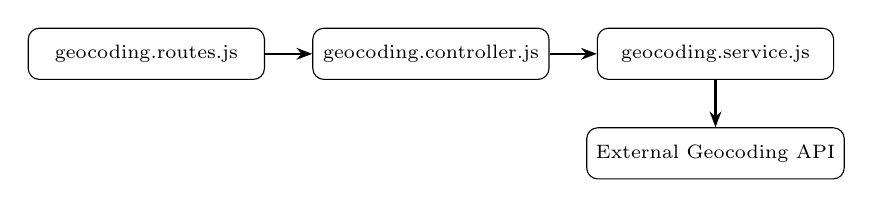
\begin{tikzpicture}[
    node distance=0.5cm and 0.6cm,
    box/.style={draw, rounded corners, minimum width=3cm, minimum height=0.65cm, align=center, font=\scriptsize},
    arrow/.style={-{Stealth[length=2mm]}, thick}
]
    \node[box] (route) {geocoding.routes.js};
    \node[box, right=of route] (ctrl) {geocoding.controller.js};
    \node[box, right=of ctrl] (svc) {geocoding.service.js};
    \node[box, below=0.6cm of svc] (api) {External Geocoding API};

    \draw[arrow] (route) -- (ctrl);
    \draw[arrow] (ctrl) -- (svc);
    \draw[arrow] (svc) -- (api);
\end{tikzpicture}
\end{center}

% ══════════════════════════════════════════════════════════════════
\section{Architectural Patterns}
% ══════════════════════════════════════════════════════════════════

The backend follows several well-known architectural patterns:

\subsection{Layered Architecture}
\begin{center}
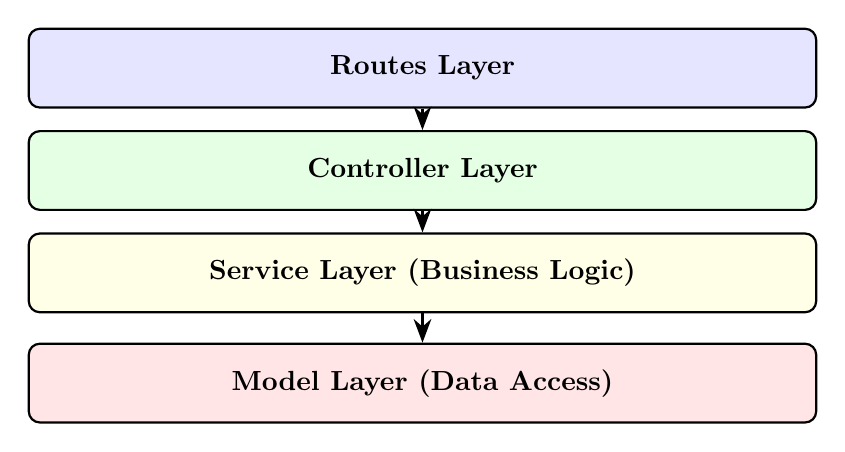
\begin{tikzpicture}[
    layer/.style={draw, thick, rounded corners, minimum width=10cm, minimum height=1cm, align=center, font=\bfseries},
    arrow/.style={-{Stealth[length=3mm]}, thick}
]
    \node[layer, fill=blue!10]   (routes)  at (0,4)  {Routes Layer};
    \node[layer, fill=green!10]  (ctrl)    at (0,2.7) {Controller Layer};
    \node[layer, fill=yellow!10] (svc)     at (0,1.4) {Service Layer (Business Logic)};
    \node[layer, fill=red!10]    (model)   at (0,0)   {Model Layer (Data Access)};

    \draw[arrow] (routes) -- (ctrl);
    \draw[arrow] (ctrl) -- (svc);
    \draw[arrow] (svc) -- (model);
\end{tikzpicture}
\end{center}

\subsection{Key Design Principles}

\begin{itemize}[leftmargin=1.5cm]
  \item \textbf{Single Responsibility Principle (SRP):} Controllers handle only HTTP request/response; services contain business logic; models define data schemas.
  \item \textbf{Dependency Inversion:} Controllers depend on service abstractions, not on direct database access.
  \item \textbf{Interface Segregation:} Routes are grouped by access level (public, authenticated, admin) so each group only uses the middleware it needs.
  \item \textbf{Open/Closed Principle:} New issue statuses can be added to \texttt{constants.js} without modifying transition logic.
\end{itemize}

% ══════════════════════════════════════════════════════════════════
\section{External Services Integration}
% ══════════════════════════════════════════════════════════════════

\begin{longtable}{@{}p{3cm}p{3cm}p{6cm}@{}}
\toprule
\textbf{Service} & \textbf{Config File} & \textbf{Purpose} \\
\midrule
\endhead
MongoDB Atlas  & \texttt{database.js}  & Primary data store via Mongoose ODM \\[4pt]
Cloudinary     & \texttt{cloudinary.config.js} & Image upload/storage for issue reports \\[4pt]
Nodemailer     & \texttt{mailer.js}    & Email notifications (SMTP) \\[4pt]
Geocoding API  & \texttt{geocoding.service.js} & Address $\leftrightarrow$ coordinate conversion \\
\bottomrule
\end{longtable}

% ══════════════════════════════════════════════════════════════════
\section{Environment Configuration}
% ══════════════════════════════════════════════════════════════════

The following environment variables are required (configured in \texttt{.env}):

\begin{longtable}{@{}p{4.5cm}p{8cm}@{}}
\toprule
\textbf{Variable} & \textbf{Description} \\
\midrule
\endhead
\texttt{PORT}                   & Server port (default: 5000) \\
\texttt{MONGODB\_URI}           & MongoDB connection string \\
\texttt{JWT\_SECRET}            & Secret key for JWT signing \\
\texttt{JWT\_EXPIRES\_IN}       & Token expiry (default: 7d) \\
\texttt{CORS\_ORIGIN}           & Allowed CORS origin (default: \texttt{http://localhost:5173}) \\
\texttt{NODE\_ENV}              & Environment mode \\
\texttt{CLOUDINARY\_CLOUD\_NAME} & Cloudinary cloud name \\
\texttt{CLOUDINARY\_API\_KEY}   & Cloudinary API key \\
\texttt{CLOUDINARY\_API\_SECRET} & Cloudinary API secret \\
\texttt{MAIL\_HOST}             & SMTP host \\
\texttt{MAIL\_PORT}             & SMTP port (default: 587) \\
\texttt{MAIL\_USER}             & SMTP username \\
\texttt{MAIL\_PASS}             & SMTP password \\
\texttt{MAIL\_FROM}             & Sender email address \\
\texttt{FRONTEND\_URL}          & Frontend application URL \\
\bottomrule
\end{longtable}

% ══════════════════════════════════════════════════════════════════
\section{Role-Based Access Control (RBAC)}
% ══════════════════════════════════════════════════════════════════

The system defines three roles with different access levels:

\begin{center}
\begin{tabular}{@{}l c c c@{}}
\toprule
\textbf{Capability} & \textbf{Citizen/User} & \textbf{Official} & \textbf{Admin} \\
\midrule
Register / Login          & \checkmark & \checkmark & \checkmark \\
View public issues        & \checkmark & \checkmark & \checkmark \\
Report a new issue        & \checkmark & \checkmark & \checkmark \\
Withdraw own issue        & \checkmark & ---        & ---        \\
Update issue status       & ---        & \checkmark & \checkmark \\
Comment on issues         & ---        & \checkmark & \checkmark \\
Create marketplace listing & \checkmark & \checkmark & \checkmark \\
Create surveys            & ---        & \checkmark & \checkmark \\
Vote on surveys           & \checkmark & \checkmark & \checkmark \\
Delete surveys            & ---        & \checkmark & \checkmark \\
Create green initiatives  & \checkmark & \checkmark & \checkmark \\
\bottomrule
\end{tabular}
\end{center}

% ══════════════════════════════════════════════════════════════════
\section{Full System Architecture Diagram}
% ══════════════════════════════════════════════════════════════════

\begin{center}
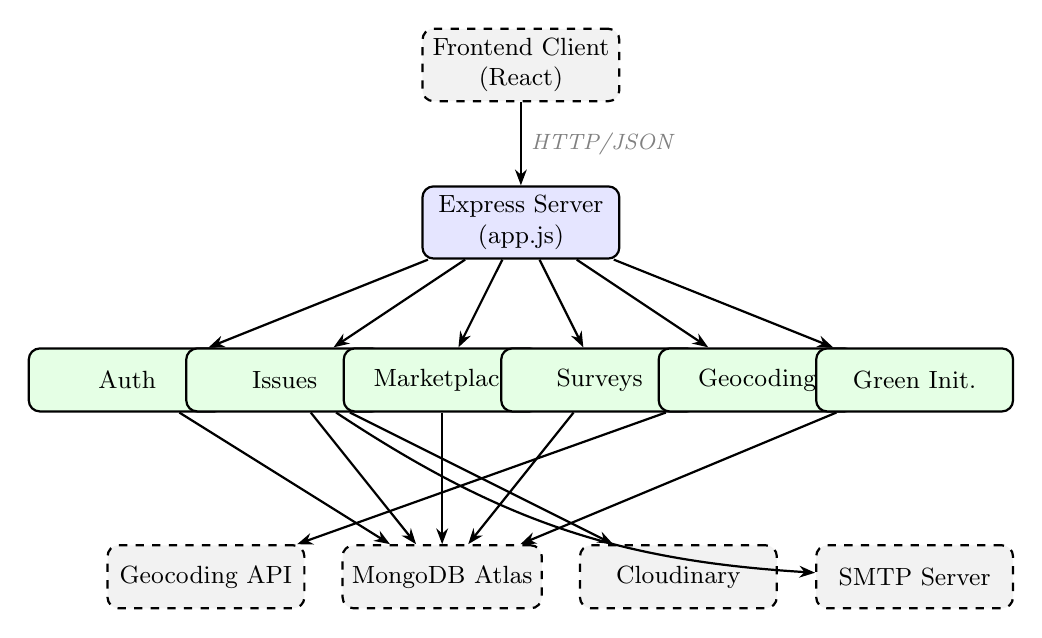
\begin{tikzpicture}[
    component/.style={draw, thick, rounded corners, minimum width=2.5cm, minimum height=0.8cm, align=center, font=\small},
    ext/.style={draw, thick, rounded corners, dashed, minimum width=2.5cm, minimum height=0.8cm, align=center, font=\small, fill=gray!10},
    arrow/.style={-{Stealth[length=2mm]}, thick},
    label/.style={font=\footnotesize\itshape, text=gray}
]
    % Client
    \node[ext] (client) at (0,6) {Frontend Client\\(React)};

    % Express Server
    \node[component, fill=blue!10] (server) at (0,4) {Express Server\\(app.js)};

    % Route modules
    \node[component, fill=green!10] (auth)   at (-5,2) {Auth};
    \node[component, fill=green!10] (issue)  at (-3,2) {Issues};
    \node[component, fill=green!10] (market) at (-1,2) {Marketplace};
    \node[component, fill=green!10] (survey) at (1,2) {Surveys};
    \node[component, fill=green!10] (geo)    at (3,2) {Geocoding};
    \node[component, fill=green!10] (green)  at (5,2) {Green Init.};

    % Data layer
    \node[ext] (mongo) at (-1,-0.5) {MongoDB Atlas};
    \node[ext] (cloud) at (2,-0.5) {Cloudinary};
    \node[ext] (mail)  at (5,-0.5) {SMTP Server};
    \node[ext] (geoapi) at (-4,-0.5) {Geocoding API};

    % Arrows
    \draw[arrow] (client) -- node[label, right]{HTTP/JSON} (server);
    \draw[arrow] (server) -- (auth);
    \draw[arrow] (server) -- (issue);
    \draw[arrow] (server) -- (market);
    \draw[arrow] (server) -- (survey);
    \draw[arrow] (server) -- (geo);
    \draw[arrow] (server) -- (green);

    \draw[arrow] (auth)   -- (mongo);
    \draw[arrow] (issue)  -- (mongo);
    \draw[arrow] (market) -- (mongo);
    \draw[arrow] (survey) -- (mongo);
    \draw[arrow] (green)  -- (mongo);

    \draw[arrow] (issue)  -- (cloud);
    \draw[arrow] (geo)    -- (geoapi);
    \draw[arrow] (issue)  to[bend right=15] (mail);
\end{tikzpicture}
\end{center}

\end{document}
